\documentclass{article}

% if you need to pass options to natbib, use, e.g.:
% \PassOptionsToPackage{numbers, compress}{natbib}
% before loading nips_2017
%
% to avoid loading the natbib package, add option nonatbib:
% \usepackage[nonatbib]{nips_2017}

%\usepackage{main}

% to compile a camera-ready version, add the [final] option, e.g.:
\usepackage[final]{main}

\usepackage[utf8]{inputenc} % allow utf-8 input
\usepackage[T1]{fontenc}    % use 8-bit T1 fonts
\usepackage{hyperref}       % hyperlinks
\usepackage{url}            % simple URL typesetting
\usepackage{booktabs}       % professional-quality tables
\usepackage{amsfonts}       % blackboard math symbols
\usepackage{nicefrac}       % compact symbols for 1/2, etc.
\usepackage{microtype}      % microtypography
\usepackage{multicol}
\usepackage{graphicx}
\usepackage{amsmath}
\usepackage{bbm}
\usepackage{enumerate}
\usepackage[linguistics]{forest}
\usepackage{adjustbox}
\usepackage{bbm}
\usepackage{stmaryrd}
\usepackage{tikz}
%\usepackage[margin=0.5in]{geometry}
%\DeclareMathOperator*{\argmax}{argmax}

\usepackage{listings}
\lstset{
  basicstyle=\ttfamily,
  mathescape
}
\usepackage{color}
 
\definecolor{codegreen}{rgb}{0,0.6,0}
\definecolor{codegray}{rgb}{0.5,0.5,0.5}
\definecolor{codepurple}{rgb}{0.58,0,0.82}
\definecolor{backcolour}{rgb}{0.95,0.95,0.92}
 
\lstdefinestyle{mystyle}{
    backgroundcolor=\color{backcolour},   
    commentstyle=\color{codegreen},
    keywordstyle=\color{magenta},
    numberstyle=\ttfamily\tiny\color{codegray},
    stringstyle=\color{codepurple},
    basicstyle=\ttfamily\small,
    columns=fullflexible,
    breakatwhitespace=false,         
    breaklines=true,                 
    captionpos=t,                    
    keepspaces=true,                 
    numbers=left,                    
    numbersep=5pt,                  
    showspaces=false,                
    showstringspaces=false,
    showtabs=false,                  
    tabsize=4,
}
 
\lstset{style=mystyle}

\title{Fundamental Algorithms - Spring 2018\\
       \Large Homework 9}
\graphicspath{{images/}}
\setcitestyle{round, sort, numbers}

% The \author macro works with any number of authors. There are two
% commands used to separate the names and addresses of multiple
% authors: \And and \AND.
%
% Using \And between authors leaves it to LaTeX to determine where to
% break the lines. Using \AND forces a line break at that point. So,
% if LaTeX puts 3 of 4 authors names on the first line, and the last
% on the second line, try using \AND instead of \And before the third
% author name.

\author{
  Daniel Rivera Ruiz\\
  Department of Computer Science\\
  New York University\\
  \href{mailto:drr342@nyu.edu}{\texttt{drr342@nyu.edu}}\\
}

\begin{document}

\maketitle

% \cite{} - in-line citation author, year in parenthesis.
% \citep{} - all citation info in parenthesis.

%	\begin{figure}[ht]
%		\centering
%		\frame{
%            \includegraphics[width=1.0\linewidth]{tree.png}
%       }
%		\caption{Classification results for the sentence \textit{"There are slow and repetitive parts, but it has just enough spice to keep it                  interesting."} using the Stanford Sentiment Treebank. As can be seen, sentiment scores are available for each phrase.}
%		\label{tree}
%	\end{figure}

\begin{enumerate}[1.]

    \item Let us define $GAP(a,b) = L - (l_a + \ldots + l_b + b - a)$ for a line that contains words with lengths $l_a$ through $l_b$. Let us now suppose that we know the value $k$ such that the words with lengths $l_k \ldots l_i$ will be in the last line of the text. The value of $FBAD[i]$ can therefore be computed as
    \begin{equation*}
        FBAD[i] = FBAD[k-1] + P[GAP(k, i)]
    \end{equation*}
    Where the value of $FBAD[k-1]$ is already known since $k \leq i$. However, we cannot know the value of $k$ a priori, and therefore we need to consider all the possible values and take the one that minimizes the previous expression. If we consider the extreme case where all words have length one, the maximum number of words that can fit in one line are $\frac{L}{2}$ (where the remaining $\frac{L}{2}$ would be occupied by white spaces between the words). Finally the formula for $FBAD[i]$ is as follows:
    \begin{equation*}
        FBAD[i] = \min_{k}\left\{FBAD[k-1] + P[GAP(k, i)]\right\}, i-\frac{L}{2} \leq k \leq i
    \end{equation*}
    The algorithm to calculate $FBAD[i]$ based on the previous formula is as follows:
\begin{lstlisting}
    FBAD[i] = $\infty$
    for k = i-$\frac{L}{2}$ to i:
        TEMP = FBAD[k-1] + P[GAP(k, i)]
        if (FBAD[i] > TEMP):
            FBAD[i] = TEMP
        end if
    end for
    return FBAD[i]
\end{lstlisting}
    We observe that all the operations inside the \texttt{for} loop take constant time and there are $\frac{L}{2}$ iterations, therefore the time complexity of the algorithm is given by $T = O\left(\frac{L}{2}\right) = O(L)$.

    \item The following image shows a representation of the graph:
    \begin{center}
        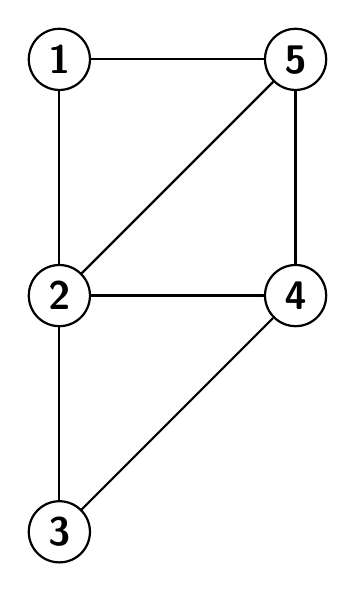
\begin{tikzpicture}[auto, node distance=3cm, every loop/.style={},
                    thick,main node/.style={circle,draw,font=\sffamily\Large\bfseries}]
        
          \node[main node] (1) {1};
          \node[main node] (2) [below of=1] {2};
          \node[main node] (3) [below of=2] {3};
          \node[main node] (4) [right of=2] {4};
          \node[main node] (5) [right of=1] {5};
        
          \path[every node/.style={font=\sffamily\small}]
            (1) edge node {} (5)
                edge node {} (2)
            (2) edge node {} (3)
                edge node {} (4)
                edge node {} (5)
            (3) edge node {} (4)
            (4) edge node {} (5);
        \end{tikzpicture}
    \end{center}
    
    The following table shows the partial results during the execution of $BFS$ with $s = 3$:
	\begin{table}[ht]
		\centering
		\begin{tabular}{cccccc}
			\toprule
			$Q$ & $u$ & $V = adj[u]$ & color$[V]$ & $d[V]$ & $\pi[V]$ \\
			\midrule
            $\{3\}$ & $3$ & $\{2,4\}$ & $\{w,w\}$ & $\{1,1\}$ & $\{3,3\}$ \\
            $\{2,4\}$ & $2$ & $\{1,5,3,4\}$ & $\{w,w,b,g\}$ & $\{2,2,-,-\}$ & $\{2,2,-,-\}$ \\
            $\{4,1,5\}$ & $4$ & $\{2,5,3\}$ & $\{b,g,b\}$ & $\{-,-,-\}$ & $\{-,-,-\}$ \\
            $\{1,5\}$ & $1$ & $\{2,5\}$ & $\{b,g\}$ & $\{-,-\}$ & $\{-,-\}$ \\
            $\{5\}$ & $5$ & $\{4,1,2\}$ & $\{b,b,b\}$ & $\{-,-,-\}$ & $\{-,-,-\}$ \\
			\bottomrule
		\end{tabular}
    \end{table}
    
    Finally, we get the values for $d$ and $\pi$:
    \begin{align*}
        d[\{1,2,3,4,5\}] &= \{2,1,0,1,2\} \\
        \pi[\{1,2,3,4,5\}] &= \{2,3,-,3,2\}
    \end{align*}
    
    \item The following table shows the partial results during the execution of $BFS$ on the graph of figure $A$ with $s = u$:
    	\begin{table}[ht]
		\centering
		\begin{tabular}{cccccc}
			\toprule
			$Q$ & $u$ & $V = adj[u]$ & color$[V]$ & $d[V]$ & $\pi[V]$ \\
			\midrule
            $\{u\}$ & $u$ & $\{t,x,y\}$ & $\{w,w,w\}$ & $\{1,1,1\}$ & $\{u,u,u\}$ \\
            $\{t,x,y\}$ & $t$ & $\{u,w,x\}$ & $\{b,w,g\}$ & $\{-,2,-\}$ & $\{-,t,-\}$ \\
            $\{x,y,w\}$ & $x$ & $\{t,u,w,y\}$ & $\{b,b,g,g\}$ & $\{-,-,-,-\}$ & $\{-,-,-,-\}$ \\
            $\{y,w\}$ & $y$ & $\{u,x\}$ & $\{b,b\}$ & $\{-,-\}$ & $\{-,-\}$ \\
            $\{w\}$ & $w$ & $\{s,t,x\}$ & $\{w,b,b\}$ & $\{3,-,-\}$ & $\{w,-,-\}$ \\
            $\{s\}$ & $s$ & $\{r,w\}$ & $\{w,b\}$ & $\{4,-\}$ & $\{s,-\}$ \\
            $\{r\}$ & $r$ & $\{s,v\}$ & $\{b,w\}$ & $\{-,5\}$ & $\{-,r\}$ \\
            $\{v\}$ & $v$ & $\{r\}$ & $\{b\}$ & $\{-\}$ & $\{-\}$ \\
			\bottomrule
		\end{tabular}
    \end{table}
    
    Finally, we get the values for $d$ and $\pi$:
    \begin{align*}
        d[\{r,s,t,u,v,w,x,y\}] &= \{4,3,1,0,5,2,1,1\} \\
        \pi[\{r,s,t,u,v,w,x,y\}] &= \{s,w,u,-,r,t,u,u\}
    \end{align*}
    
    \item Let $L = \{v_1, v_2, \ldots , v_n\}$ be the list with all the nodes (boxers) in the graph and consider the following algorithm:
\begin{lstlisting}
    initialize():
        for i = 1 to n:
            COLOR($v_i$) $\leftarrow$ WHITE;
            TYPE($v_i$) $\leftarrow$ NULL;
        end for
    
    BFS(s):
        COLOR(s) $\leftarrow$ GRAY
        Q.PUSH(s)
        while Q $\neq \{\emptyset\}$:
            u $\leftarrow$ Q.POP()
            for all v $\in$ adj(u):
                if TYPE(v) $\neq$ NULL and TYPE(v) $\neq$ TYPE(s):
                    return FALSE
                end if
                if COLOR(v) = WHITE:
                    COLOR(v) $\leftarrow$ GRAY
                    TYPE(v) $\leftarrow$ TYPE(s)
                    Q.PUSH(v)
                end if
            end for
            COLOR(u) $\leftarrow$ BLACK
        end while
    return TRUE
    
    BFS-MASTER(L):
        initialize()
        TYPE($v_1$) $\leftarrow$ GOOD
        BFS($v_1$)
        i $\leftarrow$ 2
        while TYPE($v_i$) = GOOD
            i++
            if i > n
                return FALSE
            end if
        end while
        TYPE($v_i$) $\leftarrow$ BAD
        flag = BFS($v_i$)
        if flag = FALSE
            return FALSE
        end if
        for i = 1 to n:
            if TYPE($v_i$) = NULL
                return FALSE
            end if
        end for
        print({v | TYPE(v) = GOOD})
        print({v | TYPE(v) = BAD})
    return TRUE
\end{lstlisting}

    The algorithm works as follows:
    \begin{itemize}
        \item On line 27 we initialize the fields \texttt{COLOR} and \texttt{TYPE} for all the nodes with \texttt{WHITE} and \texttt{NULL}, respectively (see lines 1 to 5).
        \item On line 28 we assign the first node $v_1$ to type \texttt{GOOD} and run \texttt{BFS} on it. After BFS finishes, all the nodes that are reachable from $v_1$ will also have type \texttt{GOOD} (see line 18).
        \item On lines 30 to 36 we find the first element that was not reached in the previous step. If no such element exists, i.e. all the elements are reachable from $v_1$ (the graph is fully connected), the algorithm terminates and returns \texttt{FALSE}.
        \item On line 38 we run \texttt{BFS} on the node $v_i$ found in the previous step. Our version of \texttt{BFS} will return \texttt{TRUE} if it terminates successfully, and \texttt{FALSE} if at any point it encounters a node which had already been reached by the first call to \texttt{BFS($v_1$)} (see lines 13 to 15).
        \item If \texttt{BFS($v_i$)} returns \texttt{FALSE}, it means that there is at least one node that can be reached by both groups \texttt{GOOD} and \texttt{BAD}, and so the algorithm returns \texttt{FALSE} and terminates (lines 39 to 41).
        \item Finally, we run a loop over all nodes to see if they have all been reached. If at least one node was never reached, the algorithm returns \texttt{FALSE} and terminates (lines 42 to 46). Otherwise, the two sets of nodes are printed and the algorithm finishes successfully (lines 47 to 49).
    \end{itemize}
    To estimate the time complexity of the algorithm we notice that \texttt{initialize()} takes time $O(n)$, as do the \texttt{while} and \texttt{for} loops. Additionally, each call to \texttt{BFS} takes time $O(n+r)$. Since all the operations are executed sequentially, the overall time complexity for \texttt{BFS-MASTER} will be $O(n+r)$.
    
    \item Table \ref{t1} shows the evolution of the $DFS$ algorithm on the graph of figure $B$, starting at node $r$ and considering all adjacent lists to be alphabetical. To build the table, we notice that the evolution of the stack corresponds to the changes of color in the nodes of the graph: whenever a node is added to the stack its color changes from white to gray, and whenever a node is removed its color changes from gray to black. 
    
    Finally, we gather from the table the values for $d$ and $f$:
    \begin{align*}
        d[\{r,q,s,t,u,v,w,x,y,z\}] &= \{01,04,05,11,02,06,07,12,03,13\} \\
        f[\{r,q,s,t,u,v,w,x,y,z\}] &= \{20,17,10,16,19,09,08,15,18,14\}
    \end{align*}

    \item Table \ref{t2} is similar to the one from the previous exercise, in this case for the graph of figure $C$ starting at node $m$. Based on this table, \texttt{TOP-SORT} will output the vertices according to their finishing times $f[i]$ but in reverse order:
    \begin{equation*}
        \texttt{TOP-SORT}(G_C) = \{p,n,o,s,m,r,y,v,x,w,z,u,q,t\}
    \end{equation*}
    
    \item
    \begin{enumerate}[(a)]
        \item Since $G$ is a $DAG$, we can build a linear version of it where all the nodes are in a straight line in the order defined by \texttt{TOP-SORT}. Assuming that the game starts at the first node, with $n$ nodes in the line and all the edges going from left to right (because of \texttt{TOP-SORT}), there can be at most $n-1$ edges (in the case where there is an edge between all consecutive nodes) before reaching the last node in the line. Since each edge in the graph corresponds to a move in the game, it follows that the game must end after $n-1$ moves at the most.
        
        \item The following algorithm returns \texttt{VALUE[z]} when \texttt{VALUE[w]} is given for all $w \in Adj[z]$:
\begin{lstlisting}
    FIND-WINNER[z]:
        for all w $\in$ Adj[z]:
            if VALUE[w] = DOS:
                return UNO
            end if
        end for
    return DOS
\end{lstlisting}
        \begin{itemize}
            \item In the base case $Adj[z]$ is empty i.e., $z$ is a leaf and therefore the \texttt{for} loop is never executed: we return \texttt{DOS} (as explained in the assignment).
            \item If we find a node with value \texttt{DOS}, it means that Player 1 can move from $z$ to that node and assure the victory. Therefore we return \texttt{UNO} and terminate.
            \item If all the nodes in the set have value \texttt{UNO}, no matter what Player 1 does he will leave the game in a position where Player 2 can win, therefore we return \texttt{DOS}.
        \end{itemize}
        
        \item The following variation of the \texttt{DFS-VISIT} algorithm would find the winner of the game if it started at vertex $v$:
\begin{lstlisting}
    DFS-VISIT[v]:
        COLOR[v] $\leftarrow$ GRAY
        for all w $\in$ Adj[v]:
            if COLOR[w] = WHITE:
                DFS-VISIT[w]
            end if
        end for
        COLOR[v] $\leftarrow$ BLACK
        VALUE[v] $\leftarrow$ FIND-WINNER[v]
\end{lstlisting}
        The time complexity of the modified algorithm is $O(E)$ (the same as the original algorithm) because there is only one extra \texttt{for} loop (implicit in the \texttt{FIND-WINNER} routine). This loop executes at most $E$ times and therefore the asymptotic analysis remains the same.
        
    \end{enumerate}
\end{enumerate}

\begin{table}[ht]
	\centering
	\caption{}
	\label{t1}
	\begin{tabular}{cccccc}
		\toprule
		Time & Node $n$ & $M = adj[n]$ & color$[M]$ & Stack & Interpretation\\
		\midrule
		$1$ & $-$ & $\{r\}$ & $\{w\}$ & $\{r\}$ & $d[r]$\\
        $2$ & $r$ & $\{u,y\}$ & $\{w,w\}$ & $\{r,u\}$ & $d[u]$\\
        $3$ & $u$ & $\{y\}$ & $\{w\}$ & $\{r,u,y\}$ & $d[y]$\\
        $4$ & $y$ & $\{q\}$ & $\{w\}$ & $\{r,u,y,q\}$ & $d[q]$\\
        $5$ & $q$ & $\{s,t,w\}$ & $\{w,w,w\}$ & $\{r,u,y,q,s\}$ & $d[s]$\\
        $6$ & $s$ & $\{v\}$ & $\{w\}$ & $\{r,u,y,q,s,v\}$ & $d[v]$\\
        $7$ & $v$ & $\{w\}$ & $\{w\}$ & $\{r,u,y,q,s,v,w\}$ & $d[w]$\\
        $8$ & $w$ & $\{s\}$ & $\{g\}$ & $\{r,u,y,q,s,v\}$ & $f[w]$\\
        $9$ & $v$ & $\{w\}$ & $\{b\}$ & $\{r,u,y,q,s\}$ & $f[v]$\\
        $10$ & $s$ & $\{v\}$ & $\{b\}$ & $\{r,u,y,q\}$ & $f[s]$\\
        $11$ & $q$ & $\{s,t,w\}$ & $\{b,w,b\}$ & $\{r,u,y,q,t\}$ & $d[t]$\\
        $12$ & $t$ & $\{x,y\}$ & $\{w,g\}$ & $\{r,u,y,q,t,x\}$ & $d[x]$\\
        $13$ & $x$ & $\{z\}$ & $\{w\}$ & $\{r,u,y,q,t,x,z\}$ & $d[z]$\\
        $14$ & $z$ & $\{x\}$ & $\{g\}$ & $\{r,u,y,q,t,x\}$ & $f[z]$\\
        $15$ & $x$ & $\{z\}$ & $\{b\}$ & $\{r,u,y,q,t\}$ & $f[x]$\\
        $16$ & $t$ & $\{x,y\}$ & $\{b,g\}$ & $\{r,u,y,q\}$ & $f[t]$\\
        $17$ & $q$ & $\{s,t,w\}$ & $\{b,b,b\}$ & $\{r,u,y\}$ & $f[q]$\\
        $18$ & $y$ & $\{q\}$ & $\{b\}$ & $\{r,u\}$ & $f[y]$\\
        $19$ & $u$ & $\{y\}$ & $\{b\}$ & $\{r\}$ & $f[u]$\\
        $20$ & $r$ & $\{u,y\}$ & $\{b,b\}$ & $\{\}$ & $f[r]$ \\
		\bottomrule
	\end{tabular}
\end{table}    

\begin{table}[ht]
	\centering
	\caption{}
	\label{t2}
	\begin{tabular}{cccccc}
		\toprule
		Time & Node $i$ & $J = adj[i]$ & color$[J]$ & Stack & Interpretation\\
		\midrule
		$1$ & $-$ & $\{m\}$ & $\{w\}$ & $\{m\}$ & $d[m]$\\
		$2$ & $m$ & $\{q,r,x\}$ & $\{w,w,w\}$ & $\{m,q\}$ & $d[q]$\\
		$3$ & $q$ & $\{t\}$ & $\{w\}$ & $\{m,q,t\}$ & $d[t]$\\
		$4$ & $t$ & $\{\}$ & $\{\}$ & $\{m,q\}$ & $f[t]$\\
		$5$ & $q$ & $\{t\}$ & $\{b\}$ & $\{m\}$ & $f[q]$\\
		$6$ & $m$ & $\{q,r,x\}$ & $\{b,w,w\}$ & $\{m,r\}$ & $d[r]$\\
        $7$ & $r$ & $\{u,y\}$ & $\{w,w\}$ & $\{m,r,u\}$ & $d[u]$\\
        $8$ & $u$ & $\{t\}$ & $\{b\}$ & $\{m,r\}$ & $f[u]$\\
        $9$ & $r$ & $\{u,y\}$ & $\{b,w\}$ & $\{m,r,y\}$ & $d[y]$\\
        $10$ & $y$ & $\{v\}$ & $\{w\}$ & $\{m,r,y,v\}$ & $d[v]$\\
        $11$ & $v$ & $\{w\}$ & $\{w\}$ & $\{m,r,y,v,w\}$ & $d[w]$\\
        $12$ & $w$ & $\{z\}$ & $\{w\}$ & $\{m,r,y,v,w,z\}$ & $d[z]$\\
        $13$ & $z$ & $\{\}$ & $\{\}$ & $\{m,r,y,v,w\}$ & $f[z]$\\
        $14$ & $w$ & $\{z\}$ & $\{b\}$ & $\{m,r,y,v\}$ & $f[w]$\\
        $15$ & $v$ & $\{w,x\}$ & $\{b,w\}$ & $\{m,r,y,v,x\}$ & $d[x]$\\
        $16$ & $x$ & $\{\}$ & $\{\}$ & $\{m,r,y,v\}$ & $f[x]$\\
        $17$ & $v$ & $\{w,x\}$ & $\{b,b\}$ & $\{m,r,y\}$ & $f[v]$\\
        $18$ & $y$ & $\{v\}$ & $\{b\}$ & $\{m,r\}$ & $f[y]$\\
        $19$ & $r$ & $\{u,y\}$ & $\{b,b\}$ & $\{m\}$ & $f[r]$\\
		$20$ & $m$ & $\{q,r,x\}$ & $\{b,b,b\}$ & $\{\}$ & $f[m]$\\
		$21$ & $-$ & $\{n\}$ & $\{w\}$ & $\{n\}$ & $d[n]$\\
		$22$ & $n$ & $\{o,q,u\}$ & $\{w,b,b\}$ & $\{n,o\}$ & $d[o]$\\
		$23$ & $o$ & $\{r,s,v\}$ & $\{b,w,b\}$ & $\{n,o,s\}$ & $d[s]$\\
		$24$ & $s$ & $\{r\}$ & $\{b\}$ & $\{n,o\}$ & $f[s]$\\
		$25$ & $o$ & $\{r,s,v\}$ & $\{b,b,b\}$ & $\{n\}$ & $f[o]$\\
		$26$ & $n$ & $\{o,q,u\}$ & $\{b,b,b\}$ & $\{\}$ & $f[n]$\\
		$27$ & $-$ & $\{p\}$ & $\{w\}$ & $\{p\}$ & $d[p]$\\
		$28$ & $p$ & $\{o,s\}$ & $\{b,b\}$ & $\{\}$ & $f[p]$\\
		\bottomrule
	\end{tabular}
\end{table}

\end{document}